\documentclass{beamer}
\usetheme{Madrid}
\usecolortheme{beaver}
\usepackage{amsmath}
\usepackage{verbatim}

\title{Markov Chains}
\subtitle{Using Eigen Value Decomposition}
\author{Tarandeep Singh}
\institute{IIT Hyderabad}
\date{\today}

\begin{document}

\begin{frame}
\titlepage
\end{frame}
\begin{comment}
\section{Introduction}

\begin{frame}

\frametitle{Markov Chains}


\end{frame}
\end{comment}
\section{The Problem}
\subsection{Problem Statement}

\begin{frame}
\frametitle{Problem Statement}
Consider a Markov Chain with state space  \{0,1,2,3,4\} and transition matrix
\begin{enumerate}
\begin{align}
P=\begin{matrix} & \begin{matrix}0&&1&&2&&3 && 4\end{matrix} \\\\ \begin{matrix}0\\\\1\\\\2\\\\3\\\\4\end{matrix} & \begin{pmatrix} 1 & 0 & 0 & 0 & 0 \\\\  1 / 3 & 1 / 3 & 1 / 3 & 0 & 0 \\\\  0 & 1 / 3 & 1 / 3 & 1 / 3 & 0 \\\\ 0 & 0 & 1 / 3 & 1 / 3 & 1 / 3 \\\\  0 & 0 & 0 & 0 & 1\end{pmatrix}\\\\ \end{matrix}
\end{align}
\end{enumerate}
Then \lim _{n \rightarrow \infty} p_{23}^{(n)} equals?
\end{frame}



\subsection{Problem Explanation}
\begin{frame}
\frametitle{What is a Markov Chain?}
\textbf{Markov process}: Random process for which the next step depends only on the present state; it has no memory of how the present state was reached.
\begin{align}
    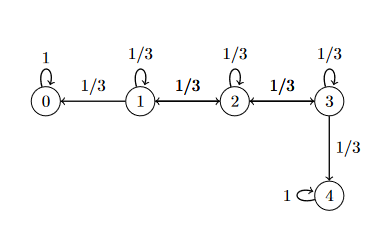
\includegraphics[scale=0.7]{state_dia.PNG}
\end{align}

\end{frame}

\section{Solution}


\begin{frame}
\frametitle{Solution}
From the given transition matrix,
\begin{align}
   p_{23}^{(1)} = P\{X_{1}=2|X_{0}=3\} = 1/3
\end{align}
This is the initial probability of reaching state 2 from state 3 as per transition matrix P. \\

\end{frame}


\begin{frame}
\frametitle{Solution}
Here, we are expected to find below,
\begin{align}
   p_{23}^{(n)} = P\{X_{n}=2|X_{0}=3\} 
\end{align}
i.e. probability of reaching state 2 after n steps from state 3.\\
In order to find $p_{ij}^{(n)}$, corresponding entry of $P^n$ matrix is required.
Matrix $P^n$ can be found easily from diagonalized form of P.  \\
\end{frame}

\begin{frame}
\frametitle{Solution} 
Using characteristic equation,
\begin{align}
    |P-\lambda I|=0
\end{align}
\begin{align}
    \left|\begin{array}{ccccc}1 - \lambda & 0 & 0 & 0 & 0\\\frac{1}{3} & \frac{1}{3} - \lambda & \frac{1}{3} & 0 & 0\\0 & \frac{1}{3} & \frac{1}{3} - \lambda & \frac{1}{3} & 0\\0 & 0 & \frac{1}{3} & \frac{1}{3} - \lambda & \frac{1}{3}\\0 & 0 & 0 & 0 & 1 - \lambda\end{array}\right| = 0
\end{align}
\end{frame}

\begin{frame}
\frametitle{Solution}
\begin{align}
\left(1-\lambda\right)^{2} \left(- \lambda^{3} + \lambda^{2} - \frac{\lambda}{9} - \frac{1}{27}\right) = 0
\end{align}
On solving, below are eigen values and corresponding eigen vectors of P
\begin{align}
\lambda_{1} = \frac{1}{3}, \left[\begin{array}{c}0\\-1\\0\\1\\0\end{array}\right] 
\lambda_{2} = 1, \left[\begin{array}{c}4\\3\\2\\1\\0\end{array}\right] \lambda_{3}=1,\left[\begin{array}{c}-3\\-2\\-1\\0\\1\end{array}\right]
\end{align}
\end{frame}

\begin{frame}
\begin{align}
\lambda_{4} = 
- \frac{-1 + \sqrt{2}}{3}, \left[\begin{array}{c}0\\1\\- \sqrt{2}\\1\\0\end{array}\right]
\lambda_{5}= 
\frac{1 + \sqrt{2}}{3},\left[\begin{array}{c}0\\1\\\sqrt{2}\\1\\0\end{array}\right]
\end{align}
Diagnolizing P from obtained eigen values and vectors,
\begin{align}
    P = X D X^{-1}
\end{align}
\end{frame}

\begin{frame}
\frametitle{Solution}
where,
\begin{align}
    D = \left[\begin{array}{ccccc}\frac{1}{3} & 0 & 0 & 0 & 0\\0 & 1 & 0 & 0 & 0\\0 & 0 & 1 & 0 & 0\\0 & 0 & 0 & - \frac{-1 + \sqrt{2}}{3} & 0\\0 & 0 & 0 & 0 & \frac{1 + \sqrt{2}}{3}\end{array}\right]
\end{align}
\begin{align}
    X = \left[\begin{array}{ccccc}0 & 4 & -3 & 2 & 0\\-1 & 3 & -2 & 1 & 1\\0 & 2 & -1 & - \sqrt{2} & \sqrt{2}\\1 & 1 & 0 & 1 & 1\\0 & 0 & 1 & 0 & 0\end{array}\right]
\end{align}
\end{frame}

\begin{frame}
\frametitle{Solution}
\begin{align}
    X^{-1} = \left[\begin{array}{ccccc}\frac{1}{4} & - \frac{1}{2} & 0 & \frac{1}{2} & - \frac{1}{4}\\\frac{1}{4} & 0 & 0 & 0 & \frac{3}{4}\\0 & 0 & 0 & 0 & 1\\\frac{-2 + \sqrt{2}}{8} & \frac{1}{4} & - \frac{\sqrt{2}}{4} & \frac{1}{4} & \frac{-2 + \sqrt{2}}{8}\\- \frac{\sqrt{2} + 2}{8} & \frac{1}{4} & \frac{\sqrt{2}}{4} & \frac{1}{4} & - \frac{\sqrt{2} + 2}{8}\end{array}\right]
\end{align}
Now,
\begin{align}
    P^{n} = X D X^{-1} \cdot X D X^{-1} \cdot X D X^{-1}..\ n\ times.
\end{align}
\begin{align}
    P^{n} = X D^{n}X^{-1}
\end{align}
\end{frame}

\begin{frame}
\frametitle{Solution}
After obtaining $X D^{n}X^{-1}$, the required entry comes out to be
\begin{align}
    P^{n}[3][2] = \frac{\sqrt{2}\left(\left(1 - \sqrt{2}\right)^{n} - \left(1 + \sqrt{2}\right)^{n}\right)}{4\cdot3^{n}} 
\end{align}
As n $\rightarrow\infty$,
\begin{align}
    P^{n}[3][2] = 0
\end{align}
Hence,
  $\lim _{n \rightarrow \infty} p_{23}^{(n)} = 0 $
\end{frame}

\begin{frame}
\frametitle{Solution}
Below figure shows change in probability wrt to n 
\begin{align}
    \includegraphics[scale=0.6]{NStepProb.PNG}
\end{align}
\end{frame}

\end{document}